\section{Basic results v2}

\begin{proposition}
  If a vertex is linked with three edges that does not share the other end, then two of those three edges are part of an alternating square.
\end{proposition}

\begin{proof}
  Among the three edges, at least two are not adjacent and thus, they need to be part of an alternating square.
\end{proof}

\begin{corollary}
  If an vertex is not part of any alternating square, then it it connected to at most two other vertices.
\end{corollary}

\begin{proposition}
  In a connected CPR graph over more than two vertices, there no triple edge outside of an alternating square and there is no double edge such that the difference between indices is not 2.
\end{proposition}

\begin{proof}
  Each end of the triple edge is not part of an alternating square and so must not be connected to more than 2 vertices. But the graph is connected, so at least one end of the graph must be connected to more than one vertex. So one end must be connected to two vertices but then the edge that connect this vertex to the new one must be adjacent to all three edges. But that is impossible.
\end{proof}

\begin{corollary}
  \label{sequence-connection}
  If a component of the permutation representation graph is composed with alternating squares. If this sequence cannot be extended it must be connected to other component of the graph by single edge.
\end{corollary}

\begin{proposition}
  \label{square-connection}
  An alternating square can be connected to a simple edge (no part of an alternating square) only if it have two adjacent simple edges with a difference in indices of exactly 2. The index of the edge used to connect the square must be between the indices of the edges of the square.
\end{proposition}

\begin{lemma}
  \label{chain-consecutive}
  In a chain, the indices must be consecutive.
\end{lemma}



\section{Basic results}

\paragraph{}
Dans la suite, nous noterons les carrés alternés grâce au deux involutions qui les composent. Un carré alterné avec des arêtes $\rho_0$ et $\rho_2$ sera noté $[\rho_0, \rho_2]$.

\begin{definition}
  Deux carrés alternés sont dit adjacents s'ils partagent deux sommets\footnote{Ces définitions sont à améliorer, il y a quelques problèmes mais je pense qu'il y a moyen de rendre ça correct}.
\end{definition}

\begin{definition}
  Une suite de carrés alternés adjacents est un suite finie dans laquelle chaque carré alterné est adjacent avec son précédesseur et son successeur s'ils existent.
\end{definition}

\begin{definition}
  Une suite de carré alternés adjacents est dite linéaire si une des deux composante de sa notation est constante.
\end{definition}

Par exemple, la suite $[\rho_0, \rho_2], [\rho_0, \rho_4], [\rho_0, \rho_3]$ est linéaire car la première composante est toujours $\rho_0$.

\begin{definition}
  Une suite de carré alterné est dite monotone si la suite formée par les différences des indices de ses carrés est monotone.
\end{definition}

La suite $[\rho_0, \rho_2], [\rho_0, \rho_3], [\rho_0, \rho_4]$ est monotone, en effet la suite formée par la différente des indice est $2, 3, 4$ et cette suite est bien monotone.

\begin{proposition}
  Toute suite de carrés alternés monotone est linéaire.
\end{proposition}

\begin{proof}
  Une suite monotone non-linéaire serait de la forme suivante: $[\rho_{i-1}, \rho_j], [\rho_i, \rho_j], [\rho_i, \rho_{j+1}]$, si nous représentons le graphe d'une telle suite nous obtenons le graphe suivant:

  \begin{figure}[H]
    \begin{center}
      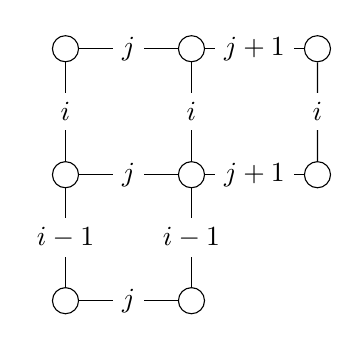
\begin{tikzpicture}[scale=.8]

        \begin{scope}[every node/.style={circle,draw}]
          \node (1)  at (0,2)  {};
          \node (2)  at (0,0)  {};
          \node (3)  at (0,-2) {};
          \node (4)  at (2,2)  {};
          \node (5)  at (2,0)  {};
          \node (6)  at (2,-2) {};
          \node (7)  at (4,2)  {};
          \node (8)  at (4,0)  {};
        \end{scope}

        \begin{scope}[every node/.style={fill=white}]

          \begin{scope}[every edge/.style={draw}]
            \path (2)  edge node {$i-1$} (3);
            \path (5)  edge node {$i-1$} (6);
            \path (1)  edge node {$i$} (2);
            \path (4)  edge node {$i$} (5);
            \path (7)  edge node {$i$} (8);
            \path (1)  edge node {$j$} (4);
            \path (2)  edge node {$j$} (5);
            \path (3)  edge node {$j$} (6);
            \path (4)  edge node {$j+1$} (7);
            \path (5)  edge node {$j+1$} (8);
          \end{scope}
        \end{scope}

      \end{tikzpicture}
      \caption{Suite de carrés alternés monotone et non-linéaire}
    \end{center}
  \end{figure}

  \paragraph{}
  Nous avons un problème en bas à droite, nous ne pouvons pas ajouter de carré à cet endroit sinon nous n'avons plus une suite, donc il faut que $i-1$ et $j+1$ soit consécutifs. On a alors $i = j+1$ ou $i+1=j$ étant donné la symétrie nous pouvons n'en conserver qu'une. Prenons $i = j+1$, ceci est un problème car alors notre carré alterné $[\rho_i, \rho_j]$ n'en est plus un, en effet $|i-j| = 1$.

\end{proof}


\begin{lemma}
  La parité de la taille d'une suite de carrés alternés est toujours la même que la partité d'une suite monotone qui admet les deux même extrémités.
\end{lemma}

\begin{lemma}
  \label{lemma-continue-alternating-square}
  Si on a un carré alterné dont les indices différent de plus 2 alors le seul moyen de l'étendre est d'utiliser un autre carré alterné.
\end{lemma}

\begin{corollary}
  Si nous travaillons sur un nombre impair de points et si nous avons un carré alterné dont la différence des indices est de plus de 2, alors toute extension de ce carré alterné à tous les points contient une suite de carrés alternés qui comprend un carré dont la différence des indices est exactement 2.
\end{corollary}

\begin{proof}
  Chaque fois que nous étendons avec un carré alterné nous ajoutons deux points. Si nous avons un nombre impair de points alors nous ne pouvons pas utiliser que des carrés alternés pour les relier. Mais si nous avons un carré alterné dont la différence des indices est de plus de deux, nous devons forcément l'étendre à un autre carré alterné. Et ainsi de suite jusqu'à avoir tous les points ou à arriver à un carré alterné dont la différence des indice ne vaut plus que deux. Le premier cas est impossible donc c'est forcément le second qui arriver.
\end{proof}

\begin{lemma}
  La taille d'une suite monotone partant du carré alterné $[i, j]$ et arrivant à une carré donc la différence des indices est 2 est $|i - j| - 2$.
\end{lemma}

\begin{lemma}
  \label{parity-sequence-squares}
  La taille d'une suite allant d'un carré alterné dont la différence des indices est 2 vers un autre carré alterné qui satisfait le même propriété est impaire.
\end{lemma}

\begin{lemma}
  \label{continue-double-edge}
  Une arête double dont la différence des indices est supérieure à 2 ne peut être relié que par un carré alterné.
\end{lemma}

\section{Intermediate results}

\begin{lemma}
  \label{lemma-forbidden-alternating-square}
  Let $\Gamma$ be sggi generating $A_{11}$ of rank 5. Then its permutation representation graph does not contains an alternating square between $\rho_0$ and $\rho_4$ if $\rho_0$ is a 4-transposition\footnote{Is this condition necessaraly?}.
\end{lemma}

\begin{proof}
  This proof and the following ones will use the same ideas to try to build valid permutation representatioin graph
  \begin{itemize}
    \item First, a pattern will be choosen and placed it on the graph (in this case, it's an alternating squre between $\rho_0$ and $\rho_4)$
    \item Then all mandatory edges will added such that the pattern can be linked to the rest of the graph
    \item All possibilities to link all the remaining points of the rest of the graph will then be tested
    \item The remaining edges will be eventually placed on the graph such that all involutions are even.
  \end{itemize}

  \paragraph{}
  If no graph were found, that mean that the pattern which has been choosen was impossible. Otherwise, this method provides a complete list of all graphs.

  \paragraph{}
  Let's start by placing the 4-transposition $\rho_4$ on the graph. We have the following graph:

  \begin{figure}[H]
    \begin{center}
      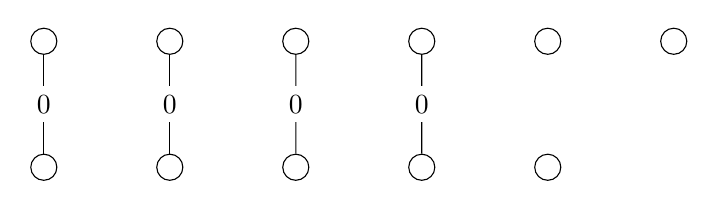
\begin{tikzpicture}[scale=.8]

        \begin{scope}[every node/.style={circle,draw}]
          \node (1)  at (0,2)  {};
          \node (2)  at (0,0)  {};
          \node (3)  at (2,2)  {};
          \node (4)  at (2,0)  {};
          \node (5)  at (4,2)  {};
          \node (6)  at (4,0)  {};
          \node (7)  at (6,2)  {};
          \node (8)  at (6,0)  {};
          \node (9)  at (8,2)  {};
          \node (10) at (8,0)  {};
          \node (11) at (10,2) {};
        \end{scope}

        \begin{scope}[every node/.style={fill=white}]

          \begin{scope}[every edge/.style={draw}]
            \path (1)  edge node {$0$} (2);
            \path (3)  edge node {$0$} (4);
            \path (5)  edge node {$0$} (6);
            \path (7)  edge node {$0$} (8);
          \end{scope}
        \end{scope}

      \end{tikzpicture}
      \caption{$\rho_0$ est une 4-transposition}
    \end{center}
  \end{figure}

  \paragraph{}
  Now, let's form an alternation square between $\rho_0$ and $\rho_4$.

  \begin{figure}[H]
    \begin{center}
      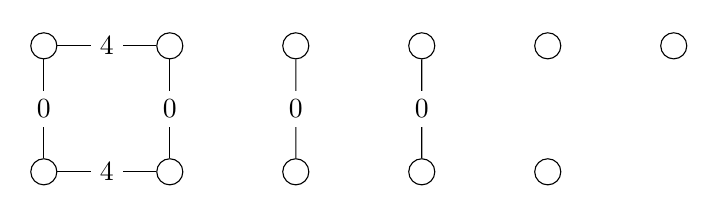
\begin{tikzpicture}[scale=.8]

        \begin{scope}[every node/.style={circle,draw}]
          \node (1)  at (0,2)  {};
          \node (2)  at (0,0)  {};
          \node (3)  at (2,2)  {};
          \node (4)  at (2,0)  {};
          \node (5)  at (4,2)  {};
          \node (6)  at (4,0)  {};
          \node (7)  at (6,2)  {};
          \node (8)  at (6,0)  {};
          \node (9)  at (8,2)  {};
          \node (10) at (8,0)  {};
          \node (11) at (10,2) {};
        \end{scope}

        \begin{scope}[every node/.style={fill=white}]

          \begin{scope}[every edge/.style={draw}]
            \path (1)  edge node {$0$} (2);
            \path (3)  edge node {$0$} (4);
            \path (5)  edge node {$0$} (6);
            \path (7)  edge node {$0$} (8);
            \path (1)  edge node {$4$} (3);
            \path (2)  edge node {$4$} (4);
          \end{scope}
        \end{scope}

      \end{tikzpicture}
      \caption{Cas 1: carré alterné}
    \end{center}
  \end{figure}

  \paragraph{}
  By Lemma~\ref{lemma-continue-alternating-square}, we need to find one sequence of alternating squares until the difference between indices is two. Therefore this sequence contains at least 3 squares. It's impossible to have 5 squares because we only have 11 points. So the sequence is monotone and so linear.

  \paragraph{}
  From the square $[\rho_0, \rho_4]$, we can go to the square $[\rho_1, \rho_4]$ or to the square $[\rho_0, \rho_3]$. But we must use the edges of involution $\rho_0$ now, the two remaining $\rho_0$ edges use 4 points and the sequence of three squares uses 8 points thus they must share at least one point. But no $\rho_0$ edge can be connected to the sequence of alternating square because an $[\rho_{-1}, \rho_1]$ square will be needed to do this but $\rho_{-1}$ does not exist. We cannot use them later in the sequence of alternating square because it is monotone and so, it will never go back to $\rho_0$ once it leave it. The only solution is that the sequence of alternating square must used a $\rho_0$ edge in the next square. The following square in the sequence is therefore $[\rho_0, \rho_3]$.

  \paragraph{}
  Because the sequence is linear, the following square must be $[\rho_0, \rho_2]$. It's the third square and the difference between indices is only two, so we can stop here. For now we have the following graph:


  \begin{figure}[H]
    \begin{center}
      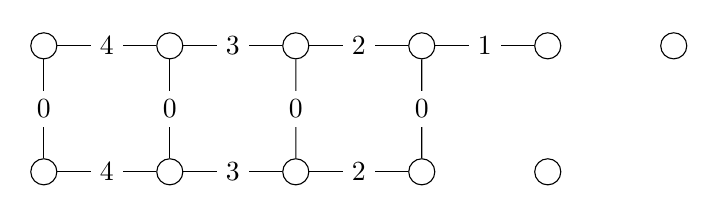
\begin{tikzpicture}[scale=.8]

        \begin{scope}[every node/.style={circle,draw}]
          \node (1)  at (0,2)  {};
          \node (2)  at (0,0)  {};
          \node (3)  at (2,2)  {};
          \node (4)  at (2,0)  {};
          \node (5)  at (4,2)  {};
          \node (6)  at (4,0)  {};
          \node (7)  at (6,2)  {};
          \node (8)  at (6,0)  {};
          \node (9)  at (8,2)  {};
          \node (10) at (8,0)  {};
          \node (11) at (10,2) {};
        \end{scope}

        \begin{scope}[every node/.style={fill=white}]

          \begin{scope}[every edge/.style={draw}]
            \path (1)  edge node {$0$} (2);
            \path (3)  edge node {$0$} (4);
            \path (5)  edge node {$0$} (6);
            \path (7)  edge node {$0$} (8);
            \path (7)  edge node {$1$} (9);
            \path (5)  edge node {$2$} (7);
            \path (6)  edge node {$2$} (8);
            \path (3)  edge node {$3$} (5);
            \path (4)  edge node {$3$} (6);
            \path (1)  edge node {$4$} (3);
            \path (2)  edge node {$4$} (4);
          \end{scope}
        \end{scope}

      \end{tikzpicture}
      \caption{Cas 1.1: doubles carrés alternés}
    \end{center}
  \end{figure}

  \paragraph{}
  To link the two remaining points, we only need two edges but the total amount of edge will be odd but that is fordidden because we want that the generated group is $A_{11}$. To restore parity we need to create a double edge or an alternating square. The number of points if insufficient to create an alternating square, so we must create a double edge and the difference between its indices must be two. All $\rho_0$ edges have already be used, so the possibilities for double edges are $(\rho_1, \rho_3)$ and $(\rho_2, \rho_4)$ but then the number of $\rho_3$ or $\rho_4$ edge becomes odd. So it is impossible to connect all points if $\rho_0$ is a 4-transposition and there is an alternating square between $\rho_0$ and $\rho_4$.
\end{proof}

\begin{lemma}
  \label{lemma-forbidden-double-edge}
  In a permutation representation graph of rank 5 with 11 points, it's impossible to have a double edge between $\rho_0$ and $\rho_4$.
\end{lemma}

\begin{proof}
  By Lemme~\ref{lemma-extend-double-edge}
  To extend a double edge $(\rho_0, \rho_4)$, we must use an alternating square, we have two possibilities, either $[\rho_0, \rho_3]$ or $[\rho_1, \rho_4]$. Those two solutions are dual, so we will only study the first one. This square must then be extended to $[\rho_0, \rho_2]$ because we must stay linear. We have the following graph:

  \begin{figure}[H]
    \begin{center}
      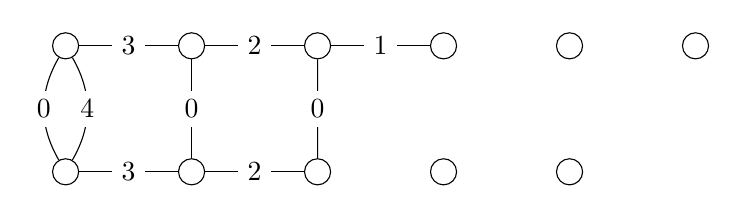
\begin{tikzpicture}[scale=.8]

        \begin{scope}[every node/.style={circle,draw}]
          \node (1)  at (0,2)  {};
          \node (2)  at (0,0)  {};
          \node (3)  at (2,2)  {};
          \node (4)  at (2,0)  {};
          \node (5)  at (4,2)  {};
          \node (6)  at (4,0)  {};
          \node (7)  at (6,2)  {};
          \node (8)  at (6,0)  {};
          \node (9)  at (8,2)  {};
          \node (10) at (8,0)  {};
          \node (11) at (10,2) {};
        \end{scope}

        \begin{scope}[every node/.style={fill=white}]

          \begin{scope}[every edge/.style={draw}]
            \path (1)  edge[bend right=30] node {$0$} (2);
            \path (3)  edge node {$0$} (4);
            \path (5)  edge node {$0$} (6);
            \path (5)  edge node {$1$} (7);
            \path (3)  edge node {$2$} (5);
            \path (4)  edge node {$2$} (6);
            \path (1)  edge node {$3$} (3);
            \path (2)  edge node {$3$} (4);
            \path (1)  edge[bend left=30] node {$4$} (2);
          \end{scope}
        \end{scope}

      \end{tikzpicture}
      \caption{Cas 1.1.2: doubles carrés alternés et arêtes doublées}
    \end{center}
  \end{figure}

  \paragraph{}
  We have two issues in this graphs: there is only one $\rho_4$ edge and if we link all remaining points with single edge, the total number of edges will be odd.

  \paragraph{}
  The $\rho_4$ edge cannot be place on the existing graph. So it must be placed between two fixed points. Then we need to link this edge to the rest of the graph, and because we have only two points, remaining, it must be done using a $\rho_2$ and $\rho_3$ edge. For now, we have the following graph:


  \begin{figure}[H]
    \begin{center}
      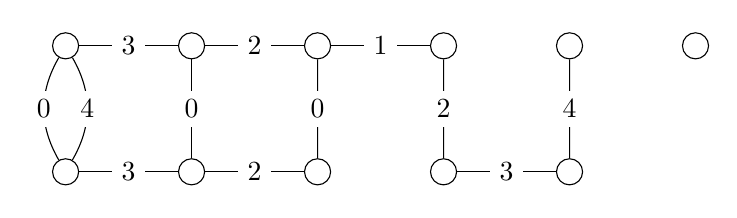
\begin{tikzpicture}[scale=.8]

        \begin{scope}[every node/.style={circle,draw}]
          \node (1)  at (0,2)  {};
          \node (2)  at (0,0)  {};
          \node (3)  at (2,2)  {};
          \node (4)  at (2,0)  {};
          \node (5)  at (4,2)  {};
          \node (6)  at (4,0)  {};
          \node (7)  at (6,2)  {};
          \node (8)  at (6,0)  {};
          \node (9)  at (8,2)  {};
          \node (10) at (8,0)  {};
          \node (11) at (10,2) {};
        \end{scope}

        \begin{scope}[every node/.style={fill=white}]

          \begin{scope}[every edge/.style={draw}]
            \path (1)  edge[bend right=30] node {$0$} (2);
            \path (3)  edge node {$0$} (4);
            \path (5)  edge node {$0$} (6);
            \path (5)  edge node {$1$} (7);
            \path (3)  edge node {$2$} (5);
            \path (4)  edge node {$2$} (6);
            \path (7)  edge node {$2$} (8);
            \path (1)  edge node {$3$} (3);
            \path (2)  edge node {$3$} (4);
            \path (8)  edge node {$3$} (10);
            \path (1)  edge[bend left=30] node {$4$} (2);
            \path (9)  edge node {$4$} (10);
          \end{scope}
        \end{scope}

      \end{tikzpicture}
      \caption{Cas 1.1.2: doubles carrés alternés et arêtes doublées}
    \end{center}
  \end{figure}

  \paragraph{}
  If wa want that the total number of point must be even, we must link the last point we a double edge. But that is impossile because the only point where we can start a double edge is the end of the $\rho_4$ edge but the the double edge must be $(\rho_3, \rho_5)$ but $\rho_5$ does not exists. Thus we cannot have a double edge between $\rho_0$ and $\rho_4$ in a permutation representation graph of $A_{11}$.


\end{proof}

\begin{corollary}
  \label{0-4-no-share}
  $\rho_0$ and $\rho_4$ edges cannot share a vertex.
\end{corollary}

\begin{proof}
  This can be directly deduced of Lemmas ~\ref{lemma-forbidden-alternating-square} and~\ref{lemma-forbidden-double-edge}.
\end{proof}
